\chapter{Hamiltonian Paths and Cycles}

Ajur walked with Jura, thinking what he could do to inspire a problem to be named after him. Rishnak found Ajur to be an interesting individual to discuss puzzles based on graph theory with. After the discussion of the Eulerian walk, Rishnak decided to introduce a closely related graph-theoretic construction, the concepts of Hamiltonian paths and Hamiltonian cycles.

Rishnak appeared in front of Ajur and immediately began defining the notion of a Hamiltonian path. ``In what's called a Hamiltonian path, each of the vertices of the given graph are visited exactly once. The length of such a path is the number of edges in that path. So, Ajur, what is the length of a Hamiltonian path in a graph with $n$ vertices?''

Ajur said, ``That's easy. A Hamiltonian path in a graph of~$n$ vertices will have a path length of~$n-1$.''

Rishank said, ``Right. And a Hamiltonian cycle is a Hamiltonian path that forms a cycle. Therefore, the length of a Hamiltonian cycle in a graph with~$n$ vertices is~$n$. Let's start with this graph.'' Rishnak presented a graph [Figure~\ref{5g1}] in the air in front of Ajur. ``Tell me, Ajur, is there a Hamiltonian cycle in this graph,\footnote{This graph is a cube graph of length~3.} and if so, what edges form the cycle?''

\begin{figure}
\begin{center}
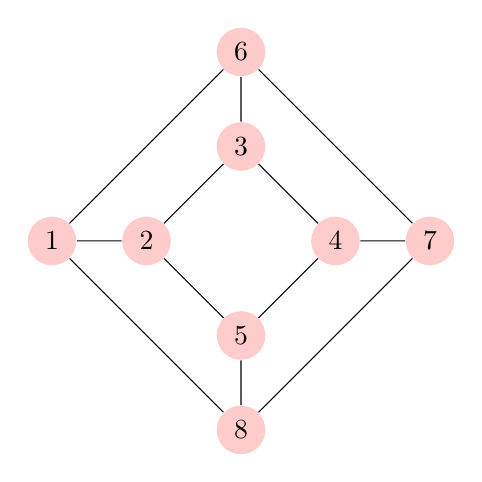
\begin{tikzpicture}
  [scale=.6,auto=left,every node/.style={circle,fill=red!20}]
  \node (n1) at (1,7) {1};
  \node (n2) at (3,7)  {2};
  \node (n4) at (7,7) {4};
  \node (n7) at (9,7)  {7};
  \node (n6) at (5,11)  {6};
   \node (n3) at (5,9) {3};
   \node (n5) at (5,5) {5};
   \node (n8)  at (5,3) {8};
  \foreach \from/\to in {n1/n2,n2/n3,n3/n4,n4/n5,n5/n2,n1/n6,
  n6/n7, n7/n8, n8/n1, n3/n6, n4/n7, n5/n8}
    \draw (\from) -- (\to);

\end{tikzpicture}
\caption{Cube graph (of length~3) with eight vertices and 12 edges}\label{5g1}
\end{center}
\end{figure}

Ajur thought about Rishnak's question for a few seconds, then picked up a stick and drew the graph and the Hamiltonian cycle in the dirt [Figure~\ref{5g2}].

Rishnak told Ajur that his solution was correct but not unique.  ``There are more solutions than just that one.\footnote{Can you find a few more Hamiltonian cycles that are different from the one described by Ajur?} And do you know why a Hamiltonian cycle is called a Hamiltonian cycle?''

Ajur frowned. ``No, but I suppose you'll tell me?''

\begin{figure}
\begin{center}
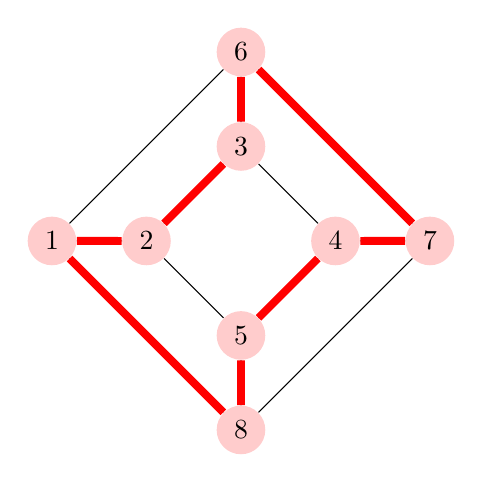
\begin{tikzpicture}
  [scale=.6,auto=left,every node/.style={circle,fill=red!20}]
  \node (n1) at (1,7) {1};
  \node (n2) at (3,7)  {2};
  \node (n4) at (7,7) {4};
  \node (n7) at (9,7)  {7};
  \node (n6) at (5,11)  {6};
   \node (n3) at (5,9) {3};
   \node (n5) at (5,5) {5};
   \node (n8)  at (5,3) {8};
  \foreach \from/\to in {n1/n2,n2/n3,n3/n4,n4/n5,n5/n2,n1/n6,
  n6/n7, n7/n8, n8/n1, n3/n6, n4/n7, n5/n8}
    \draw (\from) -- (\to);
\path[line width=1mm,red] (n1) edge (n2)
(n2) edge (n3)
(n3) edge (n6)
(n6) edge (n7)
(n7) edge (n4)
(n4) edge (n5)
(n5) edge (n8)
(n8) edge (n1);
\end{tikzpicture}
\caption{Cube graph of Figure~\ref{5g1} with a Hamiltonian cycle marked in thick edges}\label{5g2}
\end{center}
\end{figure}

Rishnak laughed and said, ``The mathematician Sir William Rowan Hamilton wanted to find a cycle to visit all of the vertices of a dodecahedron, which is a three-dimensional structure with 20 vertices and 30 edges. It's also one of the five platonic solids.''

Rishnak flashed his hands and a new graph [Figure~\ref{5g3}] appeared in dazzling lights in front of Ajur. Rishnak said, ``Is there a Hamiltonian cycle in this graph, which by the way is a well-known graph called the Petersen graph, named after mathematician Julius Petersen.''

\begin{figure}
\begin{center}
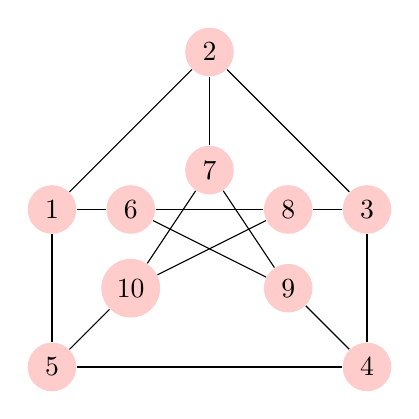
\begin{tikzpicture}
  [scale=.5,auto=left,every node/.style={circle,fill=red!20}]
  \node (n1) at (1,7) {1};
  \node (n2) at (5,11)  {2};
  \node (n3) at (9,7)  {3};
  \node (n4) at (9,3) {4};
  \node (n5) at (1,3) {5};
  \node (n6) at (3,7)  {6};
  \node (n7) at (5,8) {7};
  \node (n8)  at (7,7) {8};
  \node (n9) at (7,5) {9};
  \node (n10) at  (3,5) {10};
 
  \foreach \from/\to in {n1/n2,n2/n3,n3/n4,n4/n5,n5/n1,n1/n6,
  n2/n7, n3/n8, n4/n9, n5/n10, n6/n8, n8/n10, n10/n7,n7/n9,n9/n6}
    \draw (\from) -- (\to);

\end{tikzpicture}
\caption{The Petersen graph with 10 vertices and 15 edges}\label{5g3}
\end{center}
\end{figure}

\begin{figure}
\begin{center}
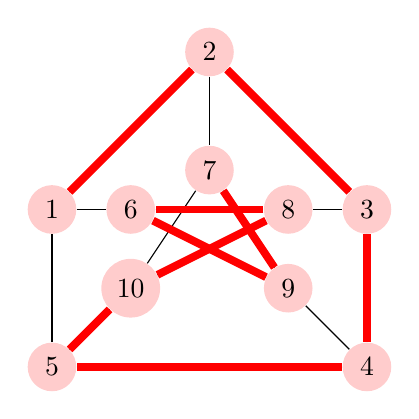
\begin{tikzpicture}
  [scale=.5,auto=left,every node/.style={circle,fill=red!20}]
  \node (n1) at (1,7) {1};
  \node (n2) at (5,11)  {2};
  \node (n3) at (9,7)  {3};
  \node (n4) at (9,3) {4};
  \node (n5) at (1,3) {5};
  \node (n6) at (3,7)  {6};
  \node (n7) at (5,8) {7};
  \node (n8)  at (7,7) {8};
  \node (n9) at (7,5) {9};
  \node (n10) at  (3,5) {10};
 
  \foreach \from/\to in {n1/n2,n2/n3,n3/n4,n4/n5,n5/n1,n1/n6,
  n2/n7, n3/n8, n4/n9, n5/n10, n6/n8, n8/n10, n10/n7,n7/n9,n9/n6}
    \draw (\from) -- (\to);
\path[line width=1mm,red]
(n1) edge (n2)
(n2) edge (n3)
(n3) edge (n4)
(n4) edge (n5)
(n5) edge (n10)
(n10) edge (n8)
(n8) edge (n6)
(n6) edge (n9)
(n9) edge (n7);

\end{tikzpicture}
\caption{The Petersen graph of Figure~\ref{5g3} with a Hamiltonian path marked in thick edges}\label{5g4}
\end{center}
\end{figure}

Ajur studied this graph for a long time, but he was not able to find a Hamiltonian cycle in the graph. He sighed and said, ``I don't see a cycle, though I do see a Hamiltonian path.''

Ajur drew the graph and a Hamiltonian path in the dirt [Figure~\ref{5g4}]. He said,  ``And that's not the only Hamiltonian path in this graph, is it?\footnote{Can you find the other Hamiltonian paths in the Petersen graph?} There are a few others.''

Rishnak smiled and assured Ajur that the Petersen graph indeed does not have a Hamiltonian cycle. He said, ``Remember the Eulerian cycle, which traverses every edge exactly once? We can easily test whether a graph has an Eulerian cycle by just testing to see whether the degree of every vertex is even. Unfortunately, there is no easy way to test whether a given graph has a Hamiltonian cycle.''

Rishnak continued, ``Speaking of cycles, there is a special class of graphs called \textit{bipartite graphs} in which every cycle is of even length. Further, in a bipartite graph, the vertex set is partitioned into two sets~$A$ and~$B$ such that every edge has one end vertex in~$A$ and its other end vertex in~$B$.''

Rishnak flashed his hands to form a new graph in the air before Ajur [Figure~\ref{5g5}].

\begin{figure}
\begin{center}
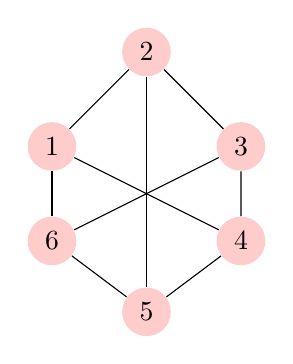
\begin{tikzpicture}
  [scale=.3,auto=left,every node/.style={circle,fill=red!20}]
  \node (n1) at (1,7) {1};
  \node (n2) at (5,11)  {2};
  \node (n3) at (9,7)  {3};
  \node (n4) at (9,3) {4};
  \node (n5) at (5,0)  {5};
  \node (n6) at (1,3) {6};
  
   \foreach \from/\to in {n1/n2,n2/n3,n3/n4,n4/n5,n5/n6,n1/n6,
  n2/n5, n6/n3,n1/n4}
    \draw (\from) -- (\to);
    \end{tikzpicture}
\caption{A bipartite graph with six vertices and nine edges, comprising vertex partition sets~$A=(1,3,5)$ and~$B=(2,4,6)$}\label{5g5}
\end{center}
\end{figure}

Ajur immediately saw that all of the cycles had even lengths, in this case~4 and~6. He said, ``And every edge in the cycle must go from one partition set to the other. These are the only possible edges. That's why the length of each cycle must be even, right?''

Rishnak nodded and asked Ajur what the two vertex partitions were for this new graph. ``All of the edges must go from one partition set to the other.''

After a little thought, Ajur said, ``One partition contains vertices~1, 3, and~5, while the other partition contains vertices~2, 4, and~6.''
He drew a new version of the graph to illustrate what he meant [Figure~\ref{5g55}].

Ajur said, ``This graph also has a Hamiltonian cycle''---he frowned, deep in thought---``Wait, every tree is a bipartite graph, too, since a tree contains no cycles. And since a tree does not have any cycles, it has no Hamiltonian cycles either.''

\begin{figure}
\begin{center}
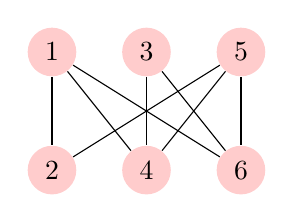
\begin{tikzpicture}
  [scale=.3,auto=left,every node/.style={circle,fill=red!20}]
  \node (n1) at (1,7) {1};
  \node (n3) at (5,7)  {3};
  \node (n5) at (9,7) {5};
  \node (n2) at (1,2)  {2};
  \node (n4) at (5,2) {4};
  \node (n6) at (9,2)  {6};
 
  
   \foreach \from/\to in {n1/n2,n1/n4,n1/n6,n3/n4,n3/n6,n5/n2,n5/n4,n5/n6}
    \draw (\from) -- (\to);
    \end{tikzpicture}
\caption{The bipartite graph from Figure~\ref{5g5} reorganized to emphasize vertex partition sets~$A=(1,3,5)$ and~$B=(2,4,6)$}\label{5g55}
\end{center}
\end{figure}

\begin{figure}
\begin{center}
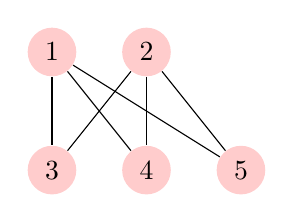
\begin{tikzpicture}
  [scale=.3,auto=left,every node/.style={circle,fill=red!20}]
  \node (n1) at (1,7) {1};
  \node (n2) at (5,7)  {2};
  \node (n3) at (1,2)  {3};
  \node (n4) at (5,2) {4};
  \node (n5) at (9,2)  {5};
 
   \foreach \from/\to in {n1/n3,n1/n4,n1/n5,n2/n3,n2/n4,n2/n5}
    \draw (\from) -- (\to);
    \end{tikzpicture}
\caption{A bipartite graph with five vertices and six edges}\label{5g6}
\end{center}
\end{figure}

Rishnak smiled.  ``That is true, Ajur. But let's get back to bipartite graphs. Can you draw a graph that is not a tree that also does not have a Hamiltonian cycle?''

Ajur wanted to show that understood these new concepts, but he struggled to see how a bipartite graph fit in here. After a few failed attempts, he said, ``Aha, I see''---he quickly drew a new graph [Figure~\ref{5g6}]---``this graph does not have a Hamiltonian cycle. If there was a Hamiltonian cycle, the vertices in the cycle would have to alternate between the two vertex partitions, but one vertex partition has only two vertices while the other vertex partition has three vertices.''

Rishnak smiled broadly, appreciating Ajur's logical thinking.  He said, ``Okay, here's another puzzle for you, Ajur. And I heard this one on the radio program Car Talk, which is broadcast on public radio.\footnote{This next problem is attributed to Bruce Robinson, a professor of Civil and Environmental Engineering at the University of Tennessee.} There are nine jealous people who live in apartments of a building that we can represent as a~$3\times3$ grid. And we can draw this a graph with each vertex representing one apartment.''

Rishnak flashed his hands to form a new graph [Figure~\ref{5g7}]. He continued, ``The apartments are numbered~1 through~9, starting in the upper left-hand corner. Each person is jealous of his adjacent neighbor, so we use edges to represent jealous neighbors wanting to move above or below, or to the right or the left. The question here is very simple. What is the fewest number of total moves that can accomplish this and make everyone happy?''

\begin{figure}
\begin{center}
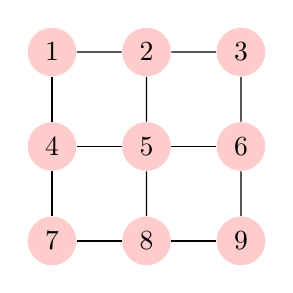
\begin{tikzpicture}
  [scale=.3,auto=left,every node/.style={circle,fill=red!20}]
  \node (n1) at (1,11) {1};
  \node (n2) at (5,11)  {2};
  \node (n3) at (9,11) {3};
  \node (n4) at (1,7)  {4};
  \node (n5) at (5,7) {5};
  \node (n6) at (9,7)  {6};
  \node (n7) at (1,3)  {7};
  \node (n8) at (5,3) {8};
  \node (n9) at (9,3)  {9};
  
  
   \foreach \from/\to in {n1/n2,n1/n4,n2/n3,n2/n5,n3/n6,n4/n5,n4/n7,n5/n6,n5/n8,n6/n9,n7/n8,
   n8/n9}
    \draw (\from) -- (\to);
    \end{tikzpicture}
\caption{A~$3\times3$ grid representing nine apartments with each apartment modeled as a vertex and each edge denoting an adjacency relation between apartments} \label{5g7}
\end{center}
\end{figure}

Ajur thought about Rishnak's question. It must have something to do with bipartite graphs. He said, ``Since there are nine vertices, the two partitions would not be of equal size. So it's not possible to have everyone move.''

Rishnak smiled and said, ``Good, but state your argument more clearly to make sure it is correct. What else can you add here?''

Ajur frowned, thinking for a minute how else he could show this to be true. At length, he said, ``The given graph has a Hamiltonian path but not a Hamiltonian cycle. So instead of a~$3\times3$ grid of apartments, if we had a~$4\times3$ grid or a~$3\times4$ grid, we would have a Hamiltonian cycle (and a bipartite graph) so it would be easy for all of them to move to an adjacent apartment.''

\newpage
Rishnak again smiled and said, ``Good, Ajur. Let's look at another problem, this one back to our friend Euler. He proposed the \textit{Knight's tour} problem on a chessboard. You probably already know a chessboard is an~$8\times8$ square grid. Place a knight in any square. From that square, the knight has to repeatedly move\footnote{To be a valid move, a knight may only move either two squares vertically up or down, then one square horizontally left or right, or one square vertically up or down, then two squares horizontally left or right. More colloquially, a knight moves in a~$2\times1$ L~shape.} and successfully visit all of the squares exactly once.''

Ajur raised his eyebrows in astonishment.

Rishnak continued, ``You may think of this problem as finding a Hamiltonian path in a 64-vertex graph with two vertices adjacent if there is a valid knight's move from one vertex to the other. There is no easy way to find a knight's tour\footnote{The solution presented in Table~\ref{5t1} is a move-by-move knight's tour for a~$5\times5$ chessboard starting from the bottom left-hand corner.} other than what's called an \textit{exhaustive} search, meaning we systematically explore every possible set of moves until we find a valid knight's tour or explore and exhaust all possibilities.''

\begin{table}
\centering
\begin{tabular}{|c |c |c| c| c|} 
 \hline
3&10&21&16& 5\\
\hline
20&15& 4&11&22\\
\hline
 9& 2&23& 6&17\\
 \hline
14&19& 8&25&12\\
\hline
 1&24&13&18& 7\\
 \hline
\end{tabular}
\caption{A valid knight's tour for a~$5\times5$ chessboard starting with move~1 at the bottom left-hand corner}
\label{5t1}
\end{table}

Ajur marveled at how one problem could be translated into another problem, then solved in a new way.

Rishnak stretched his arms out wide and a jumbling of bright letters appeared in front of Ajur [Table~\ref{5t2}]. Rishnak said, ``Can you find the message that is encoded in this grid of letters?''

\begin{table}
\centering
\begin{tabular}{c c c c cc}
i& t& t& t& b& l\\
r& h &d &e& u& s\\
h& a& y& e& d& o\\
a& o& e& p& r& n\\
s& n& f& o& l& l\\
f& v& d &i& e& u\\
\end{tabular}
\caption{Can you find the message encoded in this grid of letters?}
\label{5t2}
\end{table}

Rishnak continued, ``There are poems from different cultures, including India and China, that are actually similar to the Knight's tour problem. You can find the message by following a knight's tour.''

Ajur was intrigued and resolved to read and understand these poems. Rishnak added that one first needs to verify that a knight's tour is possible for a~$3\times3$ or~$4\times4$ chessboard. ``Be careful, though,'' warned Rishnak, ``for checking whether a knight's tour is possible may take a long time.''

Ajur asked, ``How do you mean?''

Rishnak said, ``There are many methods for checking whether a given graph has a Hamiltonian cycle. Unfortunately these conditions are not exhaustive, meaning they are not enough. Let me teach you a simple test to know whether a graph has a Hamiltonian cycle or not.''

Ajur felt his heart race in excitement.

Rishnak continued, ``A well-known theorem states that if the degree of every vertex in a graph with~$n$ vertices is at least~$\frac{n}{2}$, then the graph must have a Hamiltonian cycle. The proof consists of three parts:
\begin{enumerate}
    \item We must show that the graph is connected.
    \item The length of the longest path in any graph with~$n$ vertices is less than or equal to~$n-1$.
    \item We identify~$\mathcal{P}$ as a longest path, from which we can find a Hamiltonian cycle.''
\end{enumerate}

Ajur thought about what Rishnak had said. Quite a lot to take in and understand! Therefore, Ajur followed a systematic approach. He said, ``Okay first, the graph has to be connected. Otherwise, there would be at least two connected components, one of which would have size at most~$\frac{n}{2}$, which violates the given degree condition.''

Rishnak nodded.

Ajur continued, ``Next, in this connected graph, we need to find the longest path. Let's say we find it and it's~$v_1,v_2,\ldots,v_k$. Since this is the longest path, all neighbors of start vertex~$v_1$ and end vertex~$v_k$ must be in this path. Otherwise, we could extend that path, which would mean the path we started with was not the longest path---a contradiction.''

Rishnak nodded again.

Ajur thought about he to proceed from there, then said, ``Let's see, at least~$\frac{n}{2}$ vertices in the path~$v_2,v_3,\ldots,v_k$ are adjacent to~$v_1$. Let those adjacent vertices of~$v_1$ form set~$S_1=\{v_i,v_j,\ldots,v_m\}$. The size of this set is at least~$\frac{n}{2}$. For each of these vertices, let's then consider their preceding vertices in the path. Let that set be~$S_2$. The size of that set is also at least~$\frac{n}{2}$. Following this through, the vertices adjacent to~$v_k$ also have to be a set of size at least~$\frac{n}{2}$---and they are among~$v_1,v_2,\ldots,v_{k-1}$.''

Ajur paused. ``But if none of the vertices adjacent to~$v_k$ are in set~$S_2$, then the vertices adjacent to~$v_k$ would have size less than~$\frac{n}{2}$''---Ajur frowned, wondering how he could show this---``and we know this because~$k-1-\frac{n}{2}<\frac{n}{2}$. Aha, I see it''---Ajur drew a picture in the dirt [Figure~\ref{5g100}]---``We would have the situation shown here.''

\begin{figure}
\begin{center}
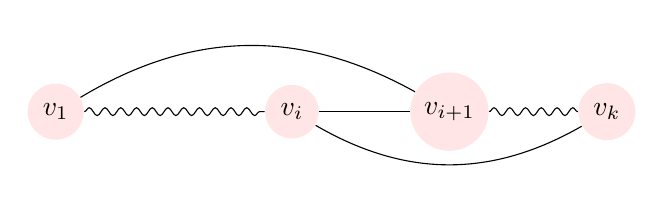
\begin{tikzpicture}
  [scale=.5,auto=left,every node/.style={circle,fill=red!10}]
  \node (n1) at (-1,11) {$v_1$};
  \node (n2) at (5,11)  {$v_i$};
  \node (n3) at (9,11) {$v_{i+1}$};
  \node (n4) at (13,11) {$v_k$};

    \draw (n2) -- (n3);
   \path (n1) edge[bend left=30] (n3);
    \path (n2) edge[bend right=30] (n4);
    \tikzset{decoration={snake,amplitude=.5mm,segment length=2mm,
                       post length=0mm,pre length=0mm}}
  \draw[decorate] (n1) -- (n2);
  \draw[decorate] (n3) -- (n4);
    \end{tikzpicture}
\caption{Graphical description of the argument used by Ajur to show that if the degree of every vertex in a graph with~$n$ vertices is at least~$\frac{n}{2}$, then the graph must have a Hamiltonian cycle; here, solid lines represent edges, whereas squiggly lines represent paths}\label{5g100}
\end{center}
\end{figure}
 
Rishnak smiled and said, ``Go on, what then?''

Ajur said, ``Then this creates cycle~$v_k,v_i,\ldots,v_1,v_{i+1}\ldots,v_k$. The claim is that this is a Hamiltonian cycle. If not, there is at least one vertex in this cycle that will be adjacent to some other vertex, but this will result in a path that is longer than the path we originally started with---a contradiction!''

Ajur jumped up and down with joy. This was a tough problem to crack and he was able to follow along. He loved the subtle and clever arguments used in the proof.

\subsection*{Question for the fifth day}
Rishnak waved his hands to form a new graph [Figure~\ref{5q1}]. He said, ``Here is a complete bipartite graph, which we can abbreviate as~$K_{2,4}$ since it has two vertices in set~$A$ and four vertices in set~$B$. More specifically, vertices~$A_1$ and~$A_2$ are adjacent to vertices~$B_3$, $B_4$, $B_5$, and~$B_6$, and there are no other edges.''

Rishnak cleared his throat, then said, ``Is there a Hamiltonian path in~$K_{2,4}$?''

\textit{Before you turn the page, try to come up with an answer of your own!}

\begin{figure}
\begin{center}
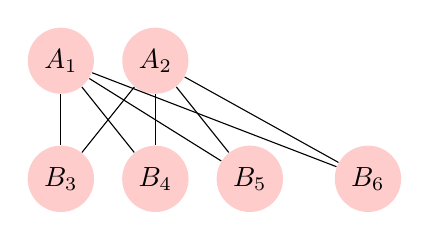
\begin{tikzpicture}
  [scale=.3,auto=left,every node/.style={circle,fill=red!20}]
  \node (n1) at (1,7) {$A_1$};
  \node (n2) at (5,7)  {$A_2$};
  \node (n3) at (1,2)  {$B_3$};
  \node (n4) at (5,2) {$B_4$};
  \node (n5) at (9,2)  {$B_5$};
  \node (n6) at (14, 2) {$B_6$};

   \foreach \from/\to in {n1/n3,n1/n4,n1/n5,n2/n3,n2/n4,n2/n5,n1/n6,n2/n6}
    \draw (\from) -- (\to);
    \end{tikzpicture}
\caption{Does complete bipartite graph~$K_{2,4}$ have a Hamiltonian path?}\label{5q1}
\end{center}
\end{figure}

\newpage
\subsection*{Answer for the fifth day}
Ajur studied the graph in front of him.  At length, he said, ``In a Hamiltonian path, vertices have to alternate between the vertices in the two different partition sets. If we start with a vertex in the larger set~$B$, then the Hamiltonian path must alternate as in~$B-A-B-A-B-A-B$, which would require there to be three vertices in partition set~$A$. Since there are only two vertices in~$A$, there cannot be a Hamiltonian path in $K_{2,4}$.''

Rishnak smiled. ``Correct.''

Ajur wanted more questions to answer and puzzles to solve, but Jura, who was patiently waiting nearby, was beginning to get restless, so Ajur decided to call it a day.
